% Author: Kailash Ranganathan
% Email: kranganathan@berkeley.edu
% CSM16A Spring 2023

\qns{Page Rank and Eigenanalysis}


\meta{
\begin{itemize}
    \item Begin by reviewing state transition graphs and matrices, and how the \textbf{matrices represent the transition from one time-step to another}. 

    \item Also ensure students \textbf{understand the concept of eigenvectors/eigenvalues} (matrices as general scaling/rotating of input vectors, and \textbf{eigenvectors as special inputs that are only scaled, not rotated})

    \item Introduce students to the concept of "eigenspaces," or the span of all a matrix's eigenvectors -- specifically, how for a full-rank matrix, \textbf{any input vector can be represented as a linear combination of eigenvectors}

    \item Perhaps this is a bit out of scope, but briefly motivate the idea of "eigenbasis" in relation to the previous bullet point -- where we conventionally think our coordinate system is defined by the 3 unit vectors, \textbf{perhaps we can just have the eigenvectors as those unit vectors; the matrix's behavior is more recognizable in the eigenbasis}

    \item The purposes of these questions are to further students' understanding of state transition diagrams by applying them to the specific scenario of webpage traffic, and to introduce how \textbf{eigenanalysis is a very useful skill outside of PageRank in determining long-term behavior of any dynamical system (important for motivation!)}
\end{itemize}}

\begin{center}
    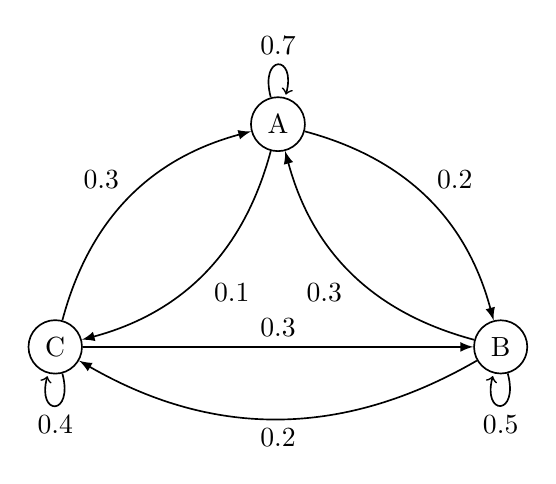
\begin{tikzpicture}[-latex, auto, node distance={4cm}, semithick, main/.style = {draw, circle}]
        \node[main] (A) {A};
        \node[main, below right of = A] (B) {B};
        \node[main, below left of = A] (C) {C}; 
        \path (A) edge[loop above] node{0.7} (A); 
        \path (A) edge[bend left] node{0.1} (C); 
        \path (A) edge[bend left] node{0.2} (B); 
        \path (B) edge[loop below] node{0.5} (B); 
        \path (B) edge[bend left] node{0.3} (A); 
        \path (B) edge[bend left] node{0.2} (C); 
        \path (C) edge node{0.3} (B); 
        \path (C) edge[bend left] node{0.3} (A); 
        \path (C) edge[loop below] node{0.4} (C); 
    \end{tikzpicture}
\end{center}

\begin{enumerate}
    \item Say we're given the state transition graph given above representing three different websites (nodes) as well as the probability users of one website move to another website (transition edges). That is, A, B, and C are all different websites, and the transition diagram above represents the flow of user traffic between them. First, write the transition matrix corresponding to the graph. Show from the matrix that the system is conservative, and explain in terms of webpages what being conservative represents. \\

    \ans{
    We first want to think of the number of people browsing each webpage at time $t$ as a vector. Lets define $x_A[t], x_B[t], x_C[t]$ as the people browsing websites A, B, and C at time $t$, and then define the "state vector" 
    \begin{equation*}
    \vec{x[t]} = \begin{bmatrix}
        x_A[t] \\
        x_B[t] \\
        x_C[t]
    \end{bmatrix}
    \end{equation*}
    With these initial steps done, we can define the state transition matrix $\textbf{T}$ satisfying $\vec{x[t+1]} = \textbf{T} \vec{x[t]}$, and by looking at the edges of the graph, populate the transition matrix values. 
    \begin{equation*}
            \textbf{T} = \begin{bmatrix}
                0.7 & 0.3 & 0.3 \\
                0.2 & 0.5 & 0.3 \\
                0.1 & 0.2 & 0.4 
            \end{bmatrix}
    \end{equation*}
    Each column sums to one, so we \textbf{have a conservative system}. What that represents for PageRank is that the number of people in this system remains constant across time--everyone browsing websites A, B, and C will all be browsing websites A, B, and C at any point in time -- there will be no net additions/subtractions of people from this "closed system" (a grim fate for the users indeed). } 

    \item Calculate one of the eigenvectors for the state transition matrix. What does the previous part tell you about (at least one of) the transition matrix's eigenvalues? Can you use this eigenvalue to quickly find its corresponding eigenvector? \\
    
    \ans{The key insight here is to notice that all conservative systems must have an eigenvalue of 1. This is because in the steady-state, the state vector converges to some non-zero vector. \par \\
    
    Lets think for a moment about what "convergence" means. This means that, at some time-step $t$, $\vec{x}[t+1] = \vec{x}[t]$. Then, compare this to our known transition equation. 
    \begin{equation*}
        \begin{split}
         & \vec{x}[t+1] = \vec{x}[t]  \\
         & \vec{x}[t+1] = \textbf{T} \vec{x}[t]
        \end{split}
    \end{equation*} 
    This means, for some $\vec{x}[t], \textbf{T}\vec{x}[t] = \vec{x}[t]$, which we can interpret as an eigenvalue equation with $\lambda = 1$. If this still is hard to understand, remove some of the notation and think about what it means for a matrix to satisfy $\textbf{A} \vec{v} = \vec{v}$.

    Going back to our original question, we now know because the system is conservative, $\textbf{T}$ has an eigenvalue $\lambda = 1.$ To find the corresponding eigenvector $\vec{v}$, we know $\textbf{T}\vec{v} = \lambda \vec{v}$, so 
    \begin{equation*}
        \textbf{T} \vec{v} - \lambda \vec{v} = 0 \xrightarrow[]{} (\textbf{T} - \lambda \textbf{I}) \vec{v} = \vec{0}
    \end{equation*}
    where $\textbf{I}$ is the identity matrix. Thus, we can calculate the above equation using $\textbf{T} - \lambda \textbf{I} = \textbf{T} - \textbf{I}$ for $\lambda = 1$ to find our eigenvector. 

    \begin{equation*}
        (\textbf{T} - \textbf{I}) \vec{v} = (\begin{bmatrix}
                0.7 & 0.3 & 0.3 \\
                0.2 & 0.5 & 0.3 \\
                0.1 & 0.2 & 0.4 
            \end{bmatrix} - \begin{bmatrix}
                1 & 0 & 0 \\
                0 & 1 & 0 \\
                0 & 0 & 1 
            \end{bmatrix}) \vec{v} = \begin{bmatrix}
                -0.3 & 0.3 & 0.3 \\
                0.2 & -0.5 & 0.3 \\
                0.1 & 0.2 & -0.6 
            \end{bmatrix} \vec{v} = \vec{0}
    \end{equation*}

    Admittedly, solving for this eigenvector is a bit mechanical. My preferred method of solving for eigenvectors is to solve for each component of the eigenvector -- that is, assume $\vec{v} = \begin{bmatrix}
        a \\
        b \\
        c 
    \end{bmatrix}$ and solve the following system of equations for each component (which you get from matrix multiplication)
    \begin{equation*}
    \begin{split}
    & -0.3a + 0.3b + 0.3c = 0 \\
    & 0.2a - 0.5b + 0.3c = 0 \\
    & 0.1a + 0.2b - 0.6c = 0 
    \end{split}
    \end{equation*}
    We get that $a = 8t, b = 5t, c = 3t$ for any arbitrary $t \neq 0$ (this set of equations has infinite solutions, as the eigenvector is really an "eigenspace"). This corresponds to $\vec{v} = t \begin{bmatrix}
        8 \\
        5 \\
        3
    \end{bmatrix}$ for arbitrary $t$, but we just need to choose one for an answer (any one is fine). 
    
    For simplicity, set $t = 1$, in which case we get the eigenvector is $\boxed{\vec{v} = \begin{bmatrix}
        8\\
        5\\
        3
    \end{bmatrix}}$ Note that this is not the only solution, as any vector that's a multiple of this $\vec{v}$ is also an eigenvector!
    }

    \item Assume the state transition matrix has three distinct eigenvalues, $\lambda_1, \lambda_2, \lambda_3$ (which, in fact, it does). Given the previous part, you already know one eigenvalue. What constraints can you put on the other two eigenvalues? 
    \emph{Hint: This is a more conceptual question -- think about the concept of eigenvalues and conservative system. As you take this system to its long-term steady-state, what must be true? }

    \ans {
    For this question, we really want to understand what the effect of differently-sized eigenvalues are on the long-term behavior of a system. We know our system is conservative, meaning the total number of people browsing pages must remain constant over time. We already know one of our eigenvalues is $1$, with its eigenvector corresponding to the steady-state behavior. 
    
    \par Suppose we had other eigenvalues $\lambda > 1$. Then, any state vector can be written as a linear combination of our three eigenvectors -- call them $\vec{v_1}, \vec{v_2}, \vec{v_3}$. Lets then call our initial state 
    \begin{equation*}
        \vec{v_i} = c_1 \vec{v_1} + c_2 \vec{v_2} + c_3 \vec{v_3} 
    \end{equation*}
    for some arbitrary constants $c_1, c_2, c_3$. After $n$ timesteps, we'd get 
    \begin{equation*}
        \vec{v_n} = T^n \vec{v_i} = T^n (c_1 \vec{v_1} + c_2 \vec{v_2} + c_3 \vec{v_3}) = c_1 T^n \vec{v_1} + c_2 T^n \vec{v_2} + c_3 T^n \vec{v_3} = c_1 \lambda_1^n \vec{v_1} + c_2 \lambda_2^n \vec{v_2} + c_3 \lambda_3^n \vec{v_3}
    \end{equation*}
    The first equivalence comes from substituting our eigenvector representation of $\vec{v_i}$. Make sure you understand this part clearly, especially why $T^n \vec{v} = \lambda^n \vec{v}$ for eigenvectors. 
    \par If $\lambda_1 = 1$, aka our steady-state eigenvalue, we'll just get its corresponding eigenvector after a very long time (aka with large $n$). But if either $\lambda_2$ or $\lambda_3$ are larger than 1, $\lambda^n$ will blow up as $n \xrightarrow[]{} \infty$, but this means our state vectors will blow up after being multiplied by insanely large values. This breaks our condition of having a conservative system, so we cannot have any $\lambda > 1$ in conservative systems. 
    \par Hence, the other two $\boxed{\lambda_2, \lambda_3 < 1}$ (assuming distinct eigenvalues) to have a properly conservative system (their eigen-components, so to speak, will diminish to zero as time goes on, and eventually we'll only have the steady-state eigenvector left).
    \par This was a lot of abstract, symbolic math, but be sure to understand the underlying ideas at play. We can represent any state vector as a linear combination of eigenvectors (formally, this is casting our vector into the eigen"basis" of the matrix), and our state transition matrix's eigenvalues essentially represent how each eigenvector as a component of the total state vector is scaled in each timestep. If we have $\lambda < 1$, this corresponds to scaling that \textit{decreases} magnitude, which over enough time, will diminish the component to zero. Contrastingly, $\lambda > 1$ corresponds to scaling that \textit{increases} magnitude, which over enough time, will compound its effects and increase the vector size without bound. Conservative systems lie perfectly in the middle, with $\lambda = 1$ leaving the eigenvector completely unchanged, hence our steady-state condition. 
    
    }

    \item Now, you are given that two of the eigenvalues are $\frac{2}{5}$ and $\frac{1}{5}$ for our state transition matrix. Say we have an initial state where $x_A[0] = 24$, $x_B[0] = 15, x_C[0] = 9$, where $x_A, x_B,$ and $x_C$ represent the number of people currently browsing the respective website A, B, or C. After a long time, what would be the number of people on each website? 

    \ans{
    Based on the logic of the previous part, we know the components corresponding with $\lambda = \frac{2}{5}$ and $\lambda = \frac{1}{5}$ will diminish to zero in steady-state. Hence, we only care about the component of the initial state vector corresponding with the eigenvector for $\lambda = 1$ which we calculated earlier. Conveniently, the input state vector $\vec{x}[0] = \begin{bmatrix}
        24 \\
        15 \\
        9 
    \end{bmatrix}$ is already the exact eigenvector for $\lambda_1 = 1$, because $\begin{bmatrix}
        24 \\
        15 \\
        9 
    \end{bmatrix} = 3 \begin{bmatrix}
        8 \\
        5 \\
        3
    \end{bmatrix} = 3 \vec{v_1}$, where $\vec{v_1}$ is the eigenvector we calculated in (b). Thus, our initial state will not change over transitions, so our steady state $\vec{x}[\infty] = \vec{x}[0] = \boxed{\begin{bmatrix}
        24 \\
        15 \\
        9 
    \end{bmatrix}}$. 
    
    }

    \item Now suppose we have a new system with a state transition matrix (not necessarily conservative) given by
    \begin{equation}
        \textbf{T} = \begin{bmatrix}
            0.3 & 0.6 & 0.1 \\
            0.3 & 0.3 & 0.1 \\
            0.9 & 0.2 & 0.3 
        \end{bmatrix}
    \end{equation}
    You may notice that the columns of this matrix are linearly dependent (can you notice this quickly without Gaussian elimination?). Thinking about the consequences of linearly dependent columns, determine--without extensive calculation--an eigenvalue of the matrix, along with its corresponding eigenvector. 

    \ans{
    The logic underlying this question is somewhat subtle. We want to split up our solution process into two main parts. 
    \begin{enumerate}
        \item Noticing that linear dependence of columns of a matrix imply that we have a nontrivial nullspace (ie. some non-zero vectors such that $\textbf{T} \vec{v} = 0$).
        \item The nullspace of a matrix is nothing more than the eigenvectors associated with an eigenvalue of $\lambda = 0$. 
    \end{enumerate}
    For the first part, the question gives us the fact that we have linear dependence of columns, and deriving nontrivial nullspaces from that is a consequence we've learned about in previous parts of 16A (if you don't remember why, think about what linear dependence of columns means, and how that combined with matrix multiplication might imply the existing of a non-zero nullspace). To verify linear dependence of columns, we can notice that the first column is three times the third column. \\  
    The second part is something we haven't encountered before. We can get at it by first writing down the definition of nullspace, that is, for a nonzero vector $\vec{v}$, 
    \begin{equation*}
        \textbf{T} \vec{v} = \vec{0}
    \end{equation*}
    Now, we can do a sort of clever substitution, where we notice that $\vec{0} = 0 \vec{v}$ for any $\vec{v}$, so 
    \begin{equation*}
        \textbf{T} \vec{v} = \vec{0} = 0 \vec{v}
    \end{equation*}
    But this is just an eigenvalue/vector equation with $\lambda = 0$. Hence, we know that $\lambda = 0$ is an eigenvalue of this transition matrix. Now realizing this fact, finding the eigenvector amounts to just finding the associated nullspace vectors of this matrix.  \\ 
    To find the nullspace vectors, we \textit{could} use Gaussian elimination, but there's a much faster way when you already know the linear dependence relation between columns. Knowing that the first column is three times the third column the first column, we can ignore the second column and construct a vector $\vec{v} = \begin{bmatrix}
        1 \\
        0 \\
        -3
    \end{bmatrix}$ that will cancel out the first and third columns, getting us $\vec{0}$. Any vector that's a multiple of what we just got also works as an eigenvector, but we'll just say one eigenvector of $\boxed{\lambda = 0}$ for this matrix is $\boxed{\vec{v} = \begin{bmatrix}
        1 \\
        0 \\
        -3
    \end{bmatrix}}$\\


    Additional notes: Conceptually, recognize the interrelatedness of nullspaces and eigenvectors. Nullspace vectors are just ones that map from themselves to 0 after passed through a matrix, but this is equivalent to "scaling" the vector by 0, as anything scaled by 0 will be 0. Thus, nullspaces and eigenvalues of 0 are really one and the same!

    
    } 
    

    \item Supposing the new system given by the previous part's $\textbf{T}$ matrix has two eigenvalues of $\lambda_1 = \frac{1}{10}(4 + \sqrt{14}), \lambda_2 = \frac{1}{10}(4 - \sqrt{14})$, given an initial state vector of $\vec{x[t]} = \begin{bmatrix}
        50 \\
        30 \\
        40 
    \end{bmatrix}$, what will be the steady-state state vector, ie. $\vec{x[t]} $ as $t \xrightarrow[]{} \infty$?

    \ans{
    Before starting the actual answer, as a general question-answering tip -- if you see numbers that look near impossible to work with, chance is there's a trick that lets you bypass directly working with those numbers to get the answer. This question has exactly that. \\
    We already know one eigenvalue is $0$ for this transition matrix, and just by looking at the other two eigenvalues we're given, we can notice that both of them are less than one ($\lambda_1 \approx \frac{6}{10}, \lambda_2 \approx 0$). Thus, our three eigenvalues for our matrix are all less than one. \\  Referring back to our work in the answer for (c), eigenvector components with associated $\lambda < 1$ will die off in steady-state. Thus, all three of our eigencomponents will die off in steady-state, and because any state vector can be represented as a linear combination of eigenvectors, any state vector for \textit{this} transition matrix will die off to $\vec{0}$ in steady-state. Thus, we know $\boxed{\vec{x}[\infty] = \vec{0}}$ for this question. Notice how we arrived at this without much computation, solely by looking at the magnitude of each eigenvalue! 
    }

\end{enumerate}

